\chapter{Modelli}\label{ch:modelli}
Il capitolo descrive i modelli realizzati, definendone sia le caratteristiche strutturali e topologiche che quelle computazionali.

Il paragrafo~\ref{sec:modelli:intro} fornisce un'introduzione ai modelli proposti, definendone i principi di base in relazione a quanto descritto nel capitolo~\ref{ch:background}.

Il paragrafo~\ref{sec:modelli:constr} introduce e discute i dettagli dell'estensione delle Graph\-ESN al caso costruttivo.

Nel paragrafo~\ref{sec:modelli:modelli} vengono descritti nello specifico i modelli oggetto della sperimentazione svolta, definendone le caratteristiche strutturali.

Nel paragrafo~\ref{sec:modelli:costo}, viene presentata un'analisi del costo computazionale relativo all'uso dei modelli proposti.

Infine, il paragrafo~\ref{ch:modelli:software} descrive le caratteristiche basilari dell'implementazione software dei modelli.

%%%%%%%%%%%%%%%%%%%%%%%%%%%%%%%%%%%%%%%%%%%%%%%%%%%%%%%%%%%%%%%

\section{Introduzione ai modelli}\label{sec:modelli:intro}
Tecniche, paradigmi e modelli descritti nel capitolo~\ref{ch:background}, benché appartenenti a periodi ed ambiti diversi, contribuiscono a formare i tratti distintivi dei modelli che saranno discussi nel corso del capitolo. Nel seguito saranno infatti introdotti dei modelli neurali, appartenenti all'ambito del Reservoir Computing, che adottino una strategia costruttiva nel trattamento di dati strutturati.

I modelli realizzati sono stati concepiti secondo un approccio incrementale, mirato ad introdurre e poi sfruttare l'approccio costruttivo con l'obiettivo di proporre soluzioni ad alcuni problemi aperti nell'ambito del Reservoir Computing. 
Ognuno dei modelli individua dunque nuove funzionalità specifiche, generalizzando i precedenti.

\begin{enumerate}[(i)]
\item Il modello \emph{GraphESN Constructive Flat} (GraphESN-CF) introduce una strategia costruttiva usando le GraphESN come unità computazionali. L'approccio costruttivo permette al modello di affrontare la necessità di fissare la topologia della rete a priori, particolarmente importante nel caso del Reservoir Computing data la presenza di reservoir non adattivi. Attraverso un procedimento iterativo di costruzione della rete, le GraphESN-CF sono dunque in grado di determinare il numero di unità da impiegare in maniera automatica e dipendente dal task: le singole sotto-reti vengono allenate per apprendere, e correggere, il segnale di errore commesso dalla rete, specializzandosi dunque ognuna in un sotto-task specifico, e vengono aggiunte alla rete in modo da formare una topologia \emph{flat}, che non preveda connessioni fra sotto-reti distinte.

\item Il modello \emph{GraphESN Forward} (GraphESN-FW) estende il precedente in modo da sfruttare le informazioni apprese nel corso del processo di costruzione incrementale della rete. Riprendendo la strategia della Cascade Correlation (si veda il paragrafo~\ref{sec:intro:cnn:ccorr}), in questo caso vengono aggiunte delle connessioni (in avanti, o \emph{forward}) fra l'output di ogni sotto-rete verso i readout di tutte le sotto-reti seguenti: quanto appreso da ogni sotto-rete contribuisce dunque alle fasi di learning successive, con lo scopo di semplificare la risoluzione del sotto-task affrontato. Grazie al fatto che ogni sotto-rete realizza una trasformazione non lineare dell'input, la GraphESN-FOF introduce una rete con topologia multilayer non lineare nell'ambito del Reservoir Computing.

\item Il modello \emph{GraphESN Forward Output-Feedback} (GraphESN-FOF) generalizza i due modelli precedenti introducendo uno schema output-feedback capace influenzare le dinamiche del reservoir. L'approccio costruttivo è in questo caso sfruttato per realizzare una strategia mirata ad affrontare uno dei problemi caratteristici del Reservoir Computing: l'impiego di un processo di encoding prefissato, guidato dalle caratteristiche dell'input ma non da quelle del task affrontato.\\
La topologia in questo caso si sviluppa connettendo gli output di ogni sotto-rete sia al readout che ai reservoir delle successive. I segnali di output delle sotto-reti, ottenuti tramite apprendimento ed utilizzabili sia su dati di training che su dati di test, vengono quindi introdotti all'interno del processo di codifica degli input, che pur rimanendo non adattivo beneficia di informazioni supervisionate, legate dunque al task affrontato.
\end{enumerate}

Altri aspetti caratterizzano i tre modelli realizzati.
Come appartenenti all'ambito del Reservoir Computing, i modelli fanno affidamento su una fase di learning estremamente vantaggiosa dal punto di vista computazionale, che interessa solo una parte delle connessioni della rete (si veda il capitolo~\ref{sec:intro:rc}). 
Infine, essendo estensioni delle GraphESN, i modelli proposti risultano in grado di apprendere trasduzioni strutturali generiche, che abbiano come input anche grafi non diretti o grafi diretti che presentino dei cicli (si veda il paragrafo~\ref{sec:intro:struct:gesn}).

Nel seguito i modelli verranno descritti nel dettaglio, privilegiando laddove possibile la formulazione più generale, ovvero riferendosi principalmente a GraphESN-FOF, in modo da non rendere la trattazione ridondante. Eventuali differenze specifiche, prevalentemente riferite alla topologia della rete, verranno evidenziate dove necessario.



%\begin{comment}
%Tecniche, paradigmi e modelli descritti nel capitolo~\ref{ch:background}, benché appartenenti a periodi ed ambiti diversi, hanno permesso di far emergere necessità e soluzioni che caratterizzano, ad oggi, la classe dei modelli neurali per il trattamento di domini strutturati. L'adozione di tecniche di allenamento efficienti e la capacità di trattare una classe di input che comprenda i grafi, risultano infatti essere fattori di grande importanza nella realizzazione di modelli per il trattamento di domini complessi. L'introduzione di un modello di Reservoir Computing per il l'apprendimento di trasduzioni su grafi, GraphESN, rappresenta una soluzione in grado di soddisfare entrambi i vincoli, ma presenta tuttavia alcuni limiti, tipici del Reservoir Computing.
%
%
%% costo computazionale e dominio di input
%% GraphESN risolve tutto ma ha alcuni problemi tipici del RC
%% Reservoir prefissato: chi mi dice quanto grosso?
%% Reservoir non adattivo: servono output-feedback.
%% L'approccio costruttivo offre soluzioni
%% Cosa faccio io?
%% - Introduco l'approccio costuttivo (risolvo il problema del reservoir prefissato)
%% - Sfrutto le informazioni apprese (come per CC)
%% - Sfrutto le informazioni apprese per introdurre uno schema di putput-feedback
%% ci sono altri vantaggi, tipici dell'approccio costruttivo: sotto-task specifici, politica locale nell'adattamento (caching), circoscrivere il learning a sotto-reti più piccole (vantaggio computaz)
%
%Tecniche, paradigmi e modelli descritti nel capitolo~\ref{ch:background} hanno permesso di far emergere necessità e soluzioni che caratterizzano ad oggi la classe dei modelli neurali per il trattamento di domini strutturati. 
%
%Con l'estensione del paradigma del Reservoir Computing al trattamento dei domini strutturati, tramite le GraphESN, è stato possibile realizzare modelli in grado di apprendere trasduzioni strutturali su grafi attraverso procedimenti di apprendimento poco onerosi. Nonostante l'efficienza computazionale e la classe degli input trattabili siano due fattori molto importanti nell'ambito delle Reti Neurali Ricorsive, le GraphESN mantengono tuttavia inalterate alcune delle criticità tipiche del Reservoir Computing. In particolare, la necessità di adottare reservoir prefissati e non adattivi rappresenta un limite 
%
%Nel capitolo~\ref{ch:background} 
%
%
%Nel seguito saranno dunque introdotti dei nuovi modelli neurali, appartenenti all'ambito del Reservoir Computing, che permettano di adottare una strategia costruttiva nel trattamento di dati strutturati.
%I modelli sono stati concepiti secondo un approccio incrementale, mirato ad introdurre e poi sfruttare l'approccio costruttivo. Ad ognuna delle seguenti fasi corrisponde dunque un modello distinto, in grado tuttavia di generalizzare i precedenti:
%\begin{enumerate}[(i)]
%\item Inizialmente si è introdotto l'approccio incrementale nell'ambito del Reservoir Computing attraverso la realizzazione di un modello che, estendendo le GraphESN, fosse in grado di determinare in maniera automatica la topologia e la dimensione della rete. La strategia costruttiva è stata realizzata utilizzando più GraphESN distinte, aggiunte in maniera incrementale e non connesse fra loro.\\
%L'adozione di un approccio costruttivo ha permesso 
%\item Sfruttare le informazioni precedentemente apprese dalla rete per potenziare 
%\item Introdurre uno schema stabile di output-feedback
%\end{enumerate}
%nel seguito, per semplicità, 
%
%\end{comment}
%
%\begin{comment}
%
%La formulazione e lo sviluppo dei modelli segue un approccio incrementale:
%- introduzione dell'approccio incrementale: flat
%- sfruttare informazioni già apprese per migliorare l'apprendimento
%- sfruttare le informazioni già apprese per realizzare un meccanismo di output-feedback.
%
%Da quanto detto emergono dunque necessità e limitazioni legate all'apprendimento di trasduzioni strutturali attraverso il paradigma neurale.
%In una disciplina fortemente orientata alle applicazioni come il Machine Learning, il costo computazionale e la classe degli input trattabili rappresentano infatti degli aspetti molto rilevanti. Il paradigma del Reservoir Computing offre soluzioni efficaci per rispondere a simili necessità, ma presenta tuttavia degli elementi critici. In particolare la presenza di una porzione di rete fissata a priori, e mantenuta inalterata durante l'apprendimento, si configura come una limitazione. La determinazione della topologia di rete appropriata e l'opportunità di modificare le dinamiche dell'intera rete sulla base del problema affrontato, sono infatti limiti la cui risoluzione rimane ad oggi un problema aperto \cite{Lukosevicius:ESNwithTrainedFeedbacks,Wyffels:stableOutputFeedback,Reinhart:ReservoirRegularization}.
%L'approccio costruttivo offre tuttavia soluzioni in tal senso, proponendo una strategia efficiente per determinare la topologia della rete in maniera automatica e per sfruttare le informazioni raccolte nel corso del processo incrementale di costruzione della rete.
%
%Nel seguito verranno introdotti dei nuovi modelli neurali, appartenenti all'ambito del Reservoir Computing, che permttano di adottare una strategia costruttiva nel trattamento di dati strutturati. 
%
%L'introduzione dell'approccio costruttivo, innovativo nell'ambito del Reservoir Computing, avviene in maniera incrementale, secondo tre fasi successive, che corrispondono ad altrettanti modelli.
%
%
%
%Tecniche, paradigmi e modelli descritti nel capitolo~\ref{ch:background}, benché appartenenti a periodi ed ambiti diversi, contribuiscono a formare i tratti distintivi dei modelli che saranno discussi nel corso del capitolo. Nel seguito saranno infatti introdotti dei modelli neurali, appartenenti all'ambito del Reservoir Computing, che permettano di adottare una strategia costruttiva nel trattamento di dati strutturati.
%
%Prima di introdurre i modelli originali, oggetto del lavoro svolto, è quindi possibile identificarne alcune caratteristiche di base, rifacendosi a quanto già descritto in precedenza, in modo da meglio comprenderne i tratti distintivi e, soprattutto, le motivazioni. 
%
%L'adozione di un approccio costruttivo, innovativo nell'ambito del Reservoir Computing, ha impatto sui modelli dal punto di vista computazionale ed algoritmico: permette la determinazione automatica della topologia della rete, la suddivisione di un task in più sotto-task, l'impiego di singole unità computazionali poco complesse e di algoritmi di apprendimento poco onerosi (si veda il paragrafo~\ref{sec:intro:cnn}). Applicata al caso del trattamento dei domini strutturati, inoltre, la strategia costruttiva offre l'opportunità di sfruttare localmente delle informazioni contestuali e supervisionate (si veda il paragrafo~\ref{sec:intro:struct}), tramite gli output-feedback, che possono essere utilizzate per influenzare le dinamiche del reservoir. 
%
%Come appartenenti all'ambito del Reservoir Computing, inoltre, i modelli sperimentati fanno affidamento su una fase di learning estremamente vantaggiosa dal punto di vista computazionale, che interessa solo una parte delle connessioni della rete (si veda il capitolo~\ref{sec:intro:rc}). 
%
%Infine, essendo estensioni delle GraphESN, i modelli proposti risultano in grado di apprendere trasduzioni strutturali generiche, che abbiano come input anche grafi non diretti o grafi diretti che presentino dei cicli (si veda il paragrafo~\ref{sec:intro:struct:gesn}).
%
%\end{comment}

%%%%%%%%%%%%%%%%%%%%%%%%%%%%%%%%%%%%%%%%%%%%%%%%%%%%%%%%%%%%%%%

\section{GraphESN costruttive}\label{sec:modelli:constr}
Stando anche a quanto descritto in precedenza (si veda il paragrafo~\vref{sec:intro:cnn}), l'approccio costruttivo prevede l'uso di singole unità computazionali, o sotto-reti, che interconnesse fra loro formano una rete nella sua totalità. Prima di poter descrivere i modelli sviluppati e definirne la topologia è dunque necessario dare una formulazione esatta di quali siano le unità di cui sono composti.

Come avviene in generale per i modelli costruttivi, consideriamo il caso in cui ogni nuova unità computazionale prenda in input gli output delle sotto-reti precedenti. Ogni sotto-rete agisce quindi come una sorta di feature-detector adattivo e la sua uscita può essere trattata come un input aggiuntivo dalle sotto-reti seguenti. Per far sì che più reti possano essere interconnesse fra loro, estendiamo reservoir e readout di una GraphESN standard in modo da rendere possibile la presenza di nuove connessioni (i.e.\ gli output di altre sotto-reti) che chiamiamo \emph{output-feedback}, provenienti da altre unità computazionali che operano indipendentemente da quella considerata.

Nel caso di trasduzioni structure-to-structure, gli output-feedback rappresentano valori calcolati in corrispondenza di ogni vertice. Il reservoir esteso della sotto-rete $i$-esima calcola, per un grafo in input $\graph{g}$ ed al passo $t$ del processo di codifica, un valore di stato $\vect{x}^{(i)}_t(v) \in \R^{N^{(i)}_R}$ per ogni vertice $v \in V(\graph{g})$ secondo la seguente equazione
\begin{equation}\label{eq:constructiveGESN:str2str}
\begin{split}	
\vect{x}^{(i)}_t(v)
	&= \tau( \vect{u}(v), \vect{x}^{(i)}_{t-1}(\mathcal{N}(v)), \vect{z}^{(1)}(v), \dots, \vect{z}^{(i-1)}(v) ) \\
	&= f( 
	\matr{W}^{(i)}_\textup{in} \, \vect{u}(v) + 
	\sum_{w \in \mathcal{N}(v)} \hat{\matr{W}}^{(i)} \, \vect{x}^{(i)}_{t-1}(w) +
	\sum_{j=1}^{i-1} \matr{W}^{(ij)}_\textup{fof} \, \vect{z}^{(j)}(v)
	)
\end{split}
\end{equation}
dove $\vect{z}^{(j)}(v) \in \R^{N^{(j)}_Z}$ rappresenta l'uscita della sotto-rete $j$-esima e $\matr{W}^{(ij)}_\textup{fof} \in \R^{N^{(i)}_R \times N^{(j)}_Z}$ è la matrice dei pesi per i (forward) output-feedback: connessioni tra il reservoir $i$-esimo e l'uscita della $j$-esima sotto-rete.

Nel caso di task structure-to-element cambia la natura degli output delle singole sotto-reti e l'equazione di transizione di stato del reservoir viene modificata di conseguenza come
\begin{equation}\label{eq:constructiveGESN:str2el}
\begin{split}	
\vect{x}^{(i)}_t(v) 
	&= \tau( \vect{u}(v), \vect{x}^{(i)}_{t-1}(\mathcal{N}(v)), \vect{z}^{(1)}(\graph{g}), \dots, \vect{z}^{(i-1)}(\graph{g}) ) \\
	&= f( 
	\matr{W}^{(i)}_\textup{in} \, \vect{u}(v) + 
	\sum_{w \in \mathcal{N}(v)} \hat{\matr{W}}^{(i)} \, \vect{x}^{(i)}_{t-1}(w) +
	\sum_{j=1}^{i-1} \matr{W}^{(ij)}_\textup{fof} \, \vect{z}^{(j)}(\graph{g})	
	)
\end{split}
\end{equation}
con $\vect{z}^{(j)}(\graph{g}) \in \R^{N^{(j)}_Z}$. 

Al netto della modifica effettuata, il processo di codifica dell'input da parte del reservoir rimane inalterato in entrambi i casi (si veda il paragrafo~\ref{sec:intro:struct:gesn} e l'algoritmo~\vref{alg:intro:gesn:reservoir}).

Il readout delle sotto-reti viene invece modificato considerando gli output-feedback come parte della codifica del grafo in input. In altri termini, la codifica viene arricchita da nuove informazioni o features che, calcolate dalle precedenti sotto-reti, vengono concatenate al vettore risultato del processo di encoding del reservoir.\\
Nel caso di trasduzioni structure-to-structure, l'uscita $\vect{z}^{(i)}(v) \in \R^{N^{(i)}_Z}$ della sotto-rete $i$-esima è quindi data da
\begin{equation}
\begin{split}
\vect{z}^{(i)}(v) 
	&= g_\textup{out}( \vect{x}^{(i)}(v), \vect{z}^{(1)}(v), \dots, \vect{z}^{(i-1)}(v) ) \\
	&= f_\textup{out}( \matr{W}^{(i)}_\textup{out} \, 
		[\vect{x}^{(i)}(v), \vect{z}^{(1)}(v), \dots, \vect{z}^{(i-1)}(v)] )
\end{split}
\end{equation}
con $[\vect{x}^{(i)}(v), \vect{z}^{(1)}(v), \dots, \vect{z}^{(i-1)}(v)]$ concatenazione della codifica corrispondente al vertice $v$ e degli output-feedback e con la matrice dei pesi del readout opportunamente modificata per adattarsi alla nuova dimensione dello spazio delle features, $\matr{W}^{(i)}_\textup{out} \in \R^{N^{(i)}_Z \times (N^{(i)}_R + \sum_{j = 1}^{i-1} N^{(j)}_Z + 1)}$.

Per le trasduzioni structure-to-element si procede in maniera simile, calcolando l'output relativo all'intero grafo $\vect{z}^{(i)}(\graph{g})$ come
\begin{equation}
\begin{split}
\vect{z}^{(i)}(\graph{g}) 
	&= g_\textup{out}( \mathcal{X}(\vect{x}^{(i)}(\graph{g})), \vect{z}^{(1)}(\graph{g}), \dots, \vect{z}^{(i-1)}(\graph{g}) ) \\
	&= f_\textup{out}( \matr{W}^{(i)}_\textup{out} \,
		[\mathcal{X}(\vect{x}^{(i)}(\graph{g})), \vect{z}^{(1)}(\graph{g}), \dots, \vect{z}^{(i-1)}(\graph{g})] )
\end{split}
\end{equation}

Poiché la natura del readout rimane sostanzialmente invariata rispetto al caso delle GraphESN, non sono necessari particolari accorgimenti per la fase di learning, che può essere eseguita con le tecniche standard.

\`E importante sottolineare alcuni aspetti relativi alla formulazione data delle singole unità computazionali.
\begin{itemize}
\item La presenza degli output-feedback è opzionale (e.g.\ $\matr{W}^{(ij)}_\textup{fof} = \vect{0}$). Questo fornisce la possibilità di implementare diverse varianti architetturali (si vedano i paragrafi~\ref{sec:modelli:constr:costruzione} e \ref{sec:modelli:modelli}) e permette di caratterizzare le singole unità computazionali come vere e proprie estensioni delle GraphESN standard. La presenza opzionale degli output-feedback determina anche il fatto che i tre modelli realizzati si generalizzino a vicenda, secondo la gerarchia descritta in precedenza nel paragrafo~\ref{sec:modelli:intro}.

\item Non è stato posto alcun vincolo particolare sulle caratteristiche di una singola unità computazionale in relazione al fatto che più sotto-reti debbano interagire fra loro. Benché ognuna sia predisposta per ricevere gli output-feedback dalle precedenti è dunque possibile che ciascuna sotto-rete differisca dalle altre nelle dimensioni del reservoir, del readout o dell'output. Questa caratteristica consente quindi l'impiego di sotto-reti eterogenee sia nelle dimensioni che nel sotto-task affrontato, permettendo la realizzazione di numerose varianti implementative.

\item I pesi dei singoli output-feedback sono tutti indipendenti l'uno dall'altro. Ne risulta un'ampia gamma di possibilità nell'implementare politiche di feedback specifiche, ad esempio facendo in modo che alcune sotto-reti abbiano maggiore influenza sulle altre (i.e.\ abbiano pesi maggiori sulle connessioni di output-feedback).

\item Gli output-feedback, agendo come input ausiliari, non modificano le condizioni per la contrattività del reservoir.
\end{itemize}
Nel seguito verrà descritto il funzionamento della rete nella sua totalità e sarà discusso in dettaglio il ruolo degli output-feedback.


%%%%%%%%%%%%%%%%%%%%%%%%%%%%%%%%%%
\subsection{Costruzione di una rete}\label{sec:modelli:constr:costruzione}
Dopo aver definito come sono fatte le singole unità che formano la rete nel suo complesso, è possibile indicare quale sia l'approccio usato per combinarle. 

Consideriamo una rete come formata da un \emph{readout globale} al quale vengono collegate in ingresso le connessioni corrispondenti alle uscite di una o più sotto-reti, aggiunte incrementalmente. Al passo $i$-esimo, ovvero dopo aver aggiunto $i$ sotto-reti, l'output della rete è dunque dato, nel caso di trasduzioni structure-to-structure, da:
\begin{equation}\label{eq:modelli:globalreadout-str2str}
\vect{y}^{(i)}(v) = f_\textup{out}( \matr{W}_\textup{out} \, [\vect{z}^{(1)}(v), \dots, \vect{z}^{(i)}(v)] )
\end{equation}
con $\matr{W}_\textup{out} \in \R^{N_Y \times (\sum_{j=1}^{i} N_Z^{(i)} + 1)}$ matrice dei pesi delle connessioni del readout globale. Nel caso dell'apprendimento di trasduzioni structure-to-element l'output è calcolato, in maniera simile, come
\begin{equation}\label{eq:modelli:globalreadout-str2el}
\vect{y}^{(i)}(\graph{g}) = f_\textup{out}( \matr{W}_\textup{out} \, [\vect{z}^{(1)}(\graph{g}), \dots, \vect{z}^{(i)}(\graph{g})] )
\end{equation}
In entrambi i casi siamo in presenza di un unico livello di connessioni che può essere allenato attraverso tecniche efficienti, in analogia con quanto avviene nelle sotto-reti ed in accordo con l'approccio del Reservoir Computing.

Internamente alla rete, ogni nuova sotto-rete può essere collegata a tutte le altre sotto-reti esistenti: gli output-feedback possono andare al reservoir della nuova sotto-rete, al suo readout o ad entrambi, in accordo con quanto descritto nel paragrafo~\ref{sec:modelli:constr}. Il modo in cui le sotto-reti sono connesse fra loro determina la differenza fra i modelli sperimentati, le cui topologie verranno descritte in seguito (si veda il paragrafo~\vref{sec:modelli:modelli}).

Ogni sotto-rete viene allenata per \emph{correggere l'errore} commesso dalla rete (i.e.\ dal readout globale). Riferendoci al caso di un task structure-to-element\footnote{Il passaggio al caso di task structure-to-structure è banale e viene quindi tralasciato per chiarezza espositiva.}, indichiamo con $\vect{e}^{(i)}(\graph{g}) \in \R^{N_Y}$ l'errore commesso dalla rete al passo $i$-esimo (i.e.\ dopo aver aggiunto $i$ sotto-reti) sull'input $\graph{g}$. La sotto-rete $(i+1)$-esima utilizza dunque $\vect{e}^{(i)}(\graph{g})$ come target nella propria fase di apprendimento. Una volta effettuato il training, la sotto-rete viene ``congelata'' ed aggiunta alla rete: il suo output diventa un nuovo input per il readout globale e può, eventualmente, essere usato come output-feedback per le sotto-reti successive. Ogni volta che una nuova unità computazionale allenata viene aggiunta alla rete si esegue un nuovo allenamento del readout globale, necessario a valutare se interrompere l'algoritmo o, in alternativa, a determinare i nuovi errori da correggere tramite ulteriori sotto-reti. 
L'allenamento del readout globale, il cui input ha una dimensionalità ridotta rispetto ai readout delle sotto-reti, ha tuttavia un costo computazionale contenuto.
L'algoritmo procede dunque iterativamente aggiungendo nuove sotto-reti e modificando l'errore, finché non venga verificato un criterio di stop prefissato (e.g.\ l'errore di training non scenda al di sotto di una soglia prefissata).

\begin{algorithm}[tb]
\caption{GraphESN costruttiva. Caso structure-to-element.}
\label{alg:modelli:constr}
\begin{algorithmic}
\STATE init sub-network counter: $i = 0$
\STATE init error: $\vect{e}^{(0)}(\graph{g}) = -\vect{y}_\textup{target}(\graph{g})$
\REPEAT
	\FORALL{$1 \leq j \leq pool\_size$}
		\STATE init $j$-th candidate
		\STATE connect candidate's output-feedback
		\STATE train candidate using $\vect{e}^{(i)}(\graph{g})$ as target 
	\ENDFOR
	\STATE select the winning candidate
	\STATE update sub-network counter: $i = i+1$
	\STATE connect the winner (i.e.\ $i$-th sub-network) to the global readout
	\STATE train the global readout
	\STATE update error $\vect{e}^{(i)}(\graph{g})$
\UNTIL{stop adding sub-networks}
\end{algorithmic}
\end{algorithm}

L'algoritmo~\vref{alg:modelli:constr} riassume il procedimento iterativo di costruzione della rete, mostrando anche come la fase di training delle sotto-reti possa avvalersi di un pool di candidate come avviene per la Cascade Correlation (si veda il paragrafo~\ref{sec:intro:cnn:ccorr}). In questo caso il pool di candidate può contenere sotto-reti che si differenziano, oltre che per l'esito dell'apprendimento, anche nell'iperparametrizzazione o nell'inizializzazione dei pesi, in particolare dei pesi del reservoir che non vengono modificati dal training.

Poiché al primo passo non è disponibile alcuna informazione sull'errore commesso, la prima sotto-rete viene allenata considerando l'errore massimo:  $\vect{e}^{(0)}(\graph{g}) = -\vect{y}_\textup{target}(\graph{g}), \forall \graph{g} \in \mathcal{G}$. Tale scelta risponde ad un'esigenza ben precisa. Il segnale appreso da una sotto-rete gioca infatti un ruolo ambivalente rispetto alla risoluzione del task: da una parte serve al readout globale come indicazione degli errori da correggere, dall'altra sposta gli stati delle sotto-reti successive in modo da raggruppare i pattern potenzialmente già corretti (si veda il paragrafo~\ref{sec:modelli:constr:outfeedback}). In quest'ottica è quindi importante che la prima sotto-rete agisca in maniera analoga alle successive, seppur riferendosi ad un errore per certi versi artificiale.

\`E infine opportuno sottolineare che la strategia incrementale adottata permette di allenare il readout globale attraverso metodi iterativi (e.g.\ LMS, si veda il paragrafo~\ref{intro:alg}). Tale pratica, comune nell'ambito delle Reti Neurali Artificiali, risulta infatti generalmente inapplicabile nel caso del Reservoir Computing a causa dell'alto numero di condizionamento delle matrici di input utilizzate per allenare quei readout che prendano i propri input direttamente da un reservoir \cite{Jaeger:ReservoirRiddles}, cosa che non avviene nel caso del readout globale, i cui input sono le uscite (precedentemente allenate) delle varie sotto-reti.



%%%%%%%%%%%%%%%%%%%%%%%%%%%%%%%%%%
\subsection{Output-feedback}\label{sec:modelli:constr:outfeedback}
Il ruolo degli output-feedback è di rilevanza centrale per i modelli proposti, in particolare rispetto al modo in cui questi possono influenzare le dinamiche del reservoir. Con riferimento al reservoir esteso dell'equazione~(\ref{eq:constructiveGESN:str2el}) è infatti importante sottolineare come i valori in $\vect{z}^{(j)}(\graph{g})$ introducano \emph{localmente} un'informazione \emph{globale}, riferita all'intero grafo in input\footnote{Nel caso di un task structure-to-structure, equazione~(\ref{eq:constructiveGESN:str2str}), è forse più corretto parlare di informazione \emph{contestuale} piuttosto che globale. Tale differenza nella terminologia è tuttavia irrilevante ai fini del discorso affrontato se non addirittura fuorviante se si considera che il processo di encoding di una GraphESN sfrutta di per sé informazioni contestuali, anche se di natura diversa da quelle qui riferite.}, e \emph{supervisionata}, ottenuta cioè tramite il processo di apprendimento (i.e.\ gli output-feedback corrispondono agli output di altre sotto-reti, precedentemente allenate). Se per la sua natura Markoviana un reservoir ha la capacità di discriminare i vertici in base ai loro vicini (ed i vicini dei vicini, e così via, iterativamente), il reservoir esteso usufruisce quindi, sia in training che in test, anche di un'informazione che gli permette di ``vedere oltre'' la frontiera che determina lo stato corrente (si veda la figura~\ref{fig:intro:encoding}) ed in base a questo di spostare gli stati in maniera consistente con il task affrontato, in funzione del target.

L'idea di sfruttare le caratteristiche dell'output per influenzare le dinamiche del reservoir è d'altra parte presente nell'ambito del Reservoir Computing sin dalla nascita delle ESN \cite{Jaeger:EchoStateApproach} e risponde all'esigenza di superare i limiti imposti dall'adozione di reservoir fissi, con dinamiche prefissate. Nonostante questo, ad oggi l'impiego di output-feedback nella loro formulazione originale comporta tecniche ed accorgimenti specifici \cite{Lukosevicius:ESNwithTrainedFeedbacks, Wyffels:stableOutputFeedback, Prokhorov:AppealAndChallenges} e presenta alcune limitazioni (si veda il paragrafo~\ref{sec:intro:rc:esn}).
I modelli proposti introducono dunque, in contrapposizione con i modelli esistenti di Reservoir Computing, un sistema di output-feedback stabile realizzato sfruttando le caratterstiche della strategia costruttiva.

Per comprenderne meglio la natura, la figura~\ref{fig:modelli:aux} mostra un esempio di come gli output-feedback possano modificare le dinamiche della rete. 
\begin{figure}[tb]
\centering
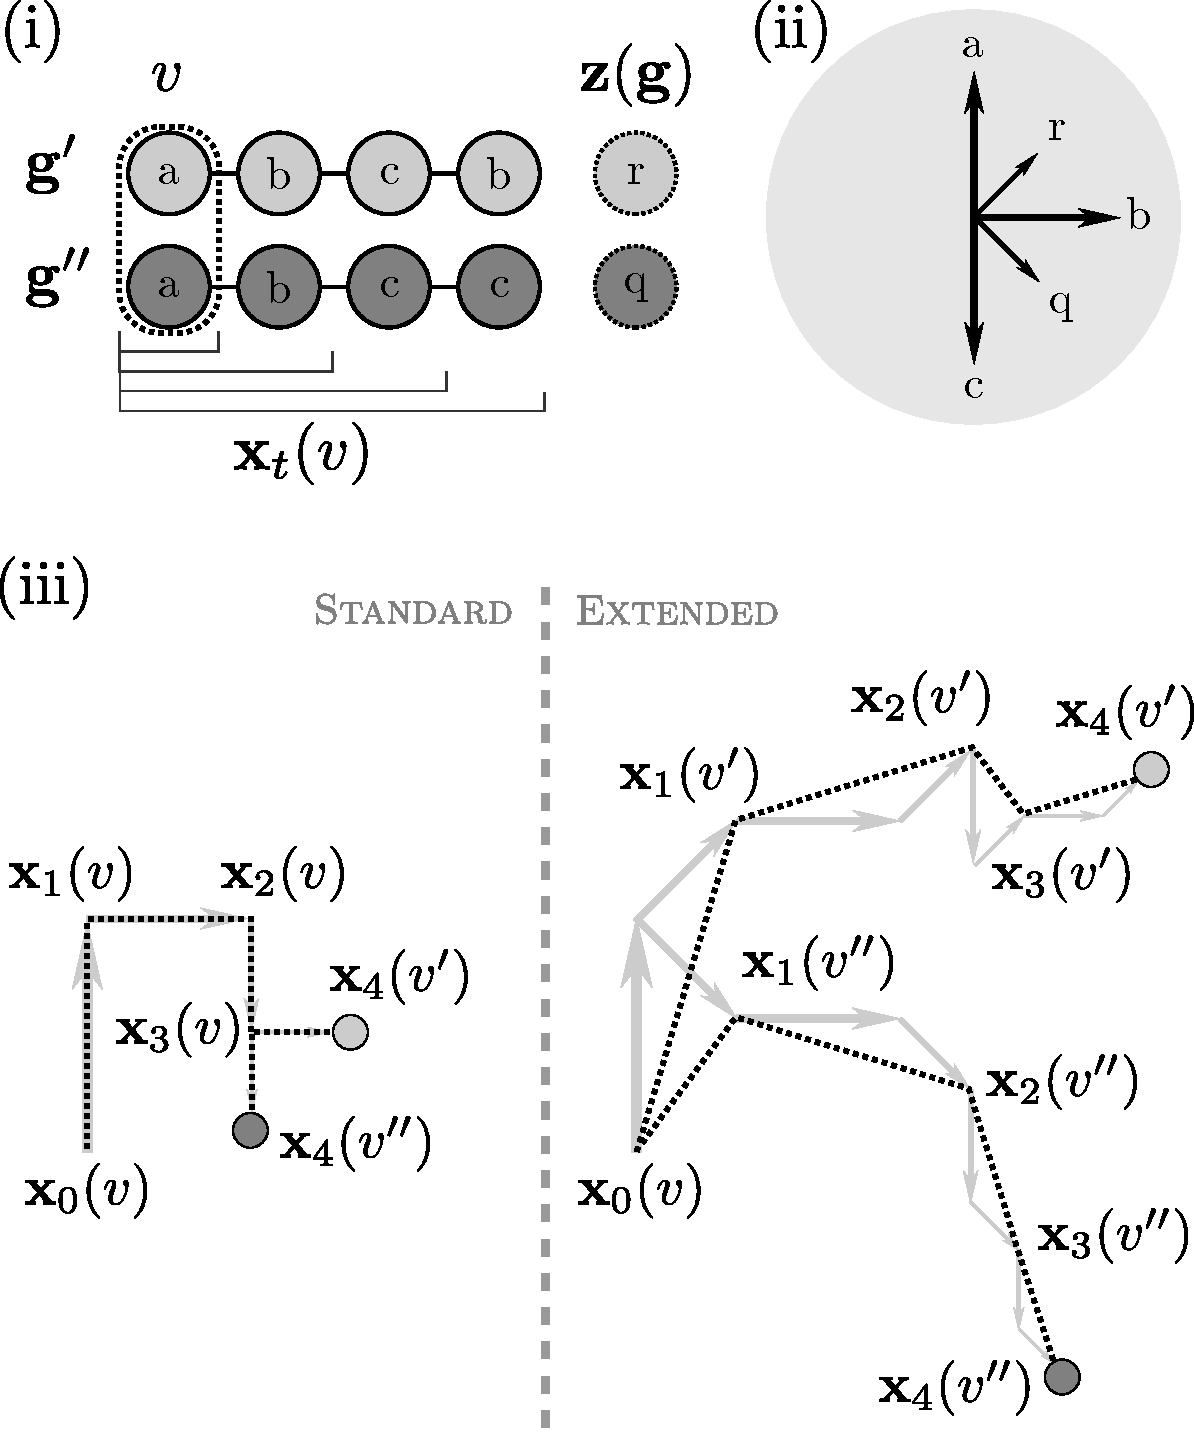
\includegraphics[width=0.65\columnwidth]{img/spazio-stati}
\medskip
\caption[Dinamiche del Reservoir esteso.]{Effetto degli output-feedback sul reservoir esteso: esempio di encoding in uno spazio bidimensionale.\\(i) Input; (ii) interpretazione geometrica degli input; (iii) traiettorie nel feature space, (\emph{sx}) reservoir standard, (\emph{dx}) reservoir esteso.}
\label{fig:modelli:aux}
\end{figure}
Con riferimento alla figura, si considerino (i) due sequenze in input $\graph{g}'$ e $\graph{g}''$, a cui siano associati target diversi (i.e.\ che debbano essere distinte dalla rete), che differiscono unicamente nell'ultimo vertice ed a cui sono associati valori di output-feedback distinti, indicati con $r$ e $q$ rispettivamente. Supponendo che lo spazio delle feature sia bidimensionale (i.e.\ $N_R = 2$), è possibile dare un'interpretazione geometrica ai vari input (e.g.\ $\matr{W}_\textup{in}\, \mathrm{a} = (0,1)$), che supponiamo essere come è indicato in (ii). In (iii) sono mostrate le traiettorie corrispondenti all'encoding iterativo del primo vertice della sequenza, indicato con $v'$ e $v''$ rispettivamente per i due input o semplicemente con $v$ quando le traiettorie nello spazio degli stati coincidono per entrambi i casi. \\
Nel caso di un un reservoir standard, a sinistra nella figura, i due input seguono la stessa traiettoria per le prime tre iterazioni. Le due sequenze sono dunque indistinguibili fino al quarto passo, ovvero fino a quando l'insieme dei vertici che determina lo stato $\vect{x}(v)$ è sufficientemente ampio da includere l'ultimo vertice. Si nota inoltre come, per effetto della natura Markoviana del reservoir, gli spostamenti delle variabili di stato si riducano con l'aumentare delle iterazioni di modo che l'ultima iterazione, quella determinante per discriminare $\graph{g}'$ e $\graph{g}''$ nel reservoir standard, mantenga comunque le due codifiche $\vect{x}_4(v')$ e $\vect{x}_4(v'')$ molto vicine nello spazio degli stati. \\
Sulla destra sono invece mostrate le traiettorie nel caso in cui ai due input sia associato un output-feedback differente, tenuto in considerazione dal reservoir esteso nel corso del processo di encoding. La figura evidenzia come in questo caso le traiettorie si differenzino sin dalla prima iterazione, permettendo di discriminare le due sequenze ben prima che l'encoding di $v'$ e $v''$ arrivi ad includere l'etichetta dell'ultimo vertice e con l'effetto di portare $\vect{x}_4(v')$ e $\vect{x}_4(v'')$ in punti molto più lontani all'interno del feature space rispetto a quanto avverrebbe con un reservoir standard.

Per effetto dello spostamento appena descritto, dunque, i pattern in input tenderanno a raggrupparsi nello spazio degli stati in maniera consistente con i propri valori degli output-feedback. \`E importante notare che, quando le varie sotto-reti sono allenate per riprodurre un segnale legato all'errore residuo commesso dalla rete (e.g.\ emulando l'errore o massimizzando la correlazione fra il proprio output e l'errore, si veda il paragrafo~\vref{sec:intro:cnn:ccorr}), allora si avrà uno spostamento maggiore in quegli input per cui sia stato precedentemente riconosciuto un alto errore residuo, e che hanno dunque maggiore probabilità di essere stati corretti dalla rete nei passi precedenti (si veda anche il paragrafo~\ref{sec:modelli:constr:costruzione}). Informalmente potremmo dire che gli output-feedback, provenienti da altre unità computazionali, hanno in questo caso l'effetto di ``mettere da parte'' gli input i cui errori siano già stati corretti da altre sotto-reti, permettendo dunque al learning di concentrarsi maggiormente su una porzione di pattern per i quali la rete commette gli errori maggiori.



%%%%%%%%%%%%%%%%%%%%%%%%%%%%%%%%%%
\section{Modelli}\label{sec:modelli:modelli}
Come detto in precedenza, i modelli sperimentati si distinguono nel modo in cui le varie sotto-reti vengono collegate fra loro. 

Mantenendo il denominatore comune dell'approccio costruttivo, secondo i principi e le modalità già descritte, i tre modelli proposti si inseriscono in un percorso incrementale che guarda all'arricchimento della struttura nelle connessioni in modo da sfruttare l'introduzione di informazione supervisionata attraverso la presenza degli output-feedback. 


\subsubsection*{GraphESN-CF}
Il modello \emph{GraphESN-CF} (i.e.\ GraphESN Constructive Flat) rappresenta l'estensione delle GraphESN al caso costruttivo: le singole sotto-reti vengono aggiunte incrementalmente ma non vi è alcuna connessione fra i loro output. Il modello è quindi formato da un unico strato di sotto-reti e dal readout globale, senza che sia presente alcun output-feedback.

La figura~\vref{fig:modelli:cf} mostra schematicamente la topologia del modello GraphESN-CF.
\begin{figure}[tb]
\centering
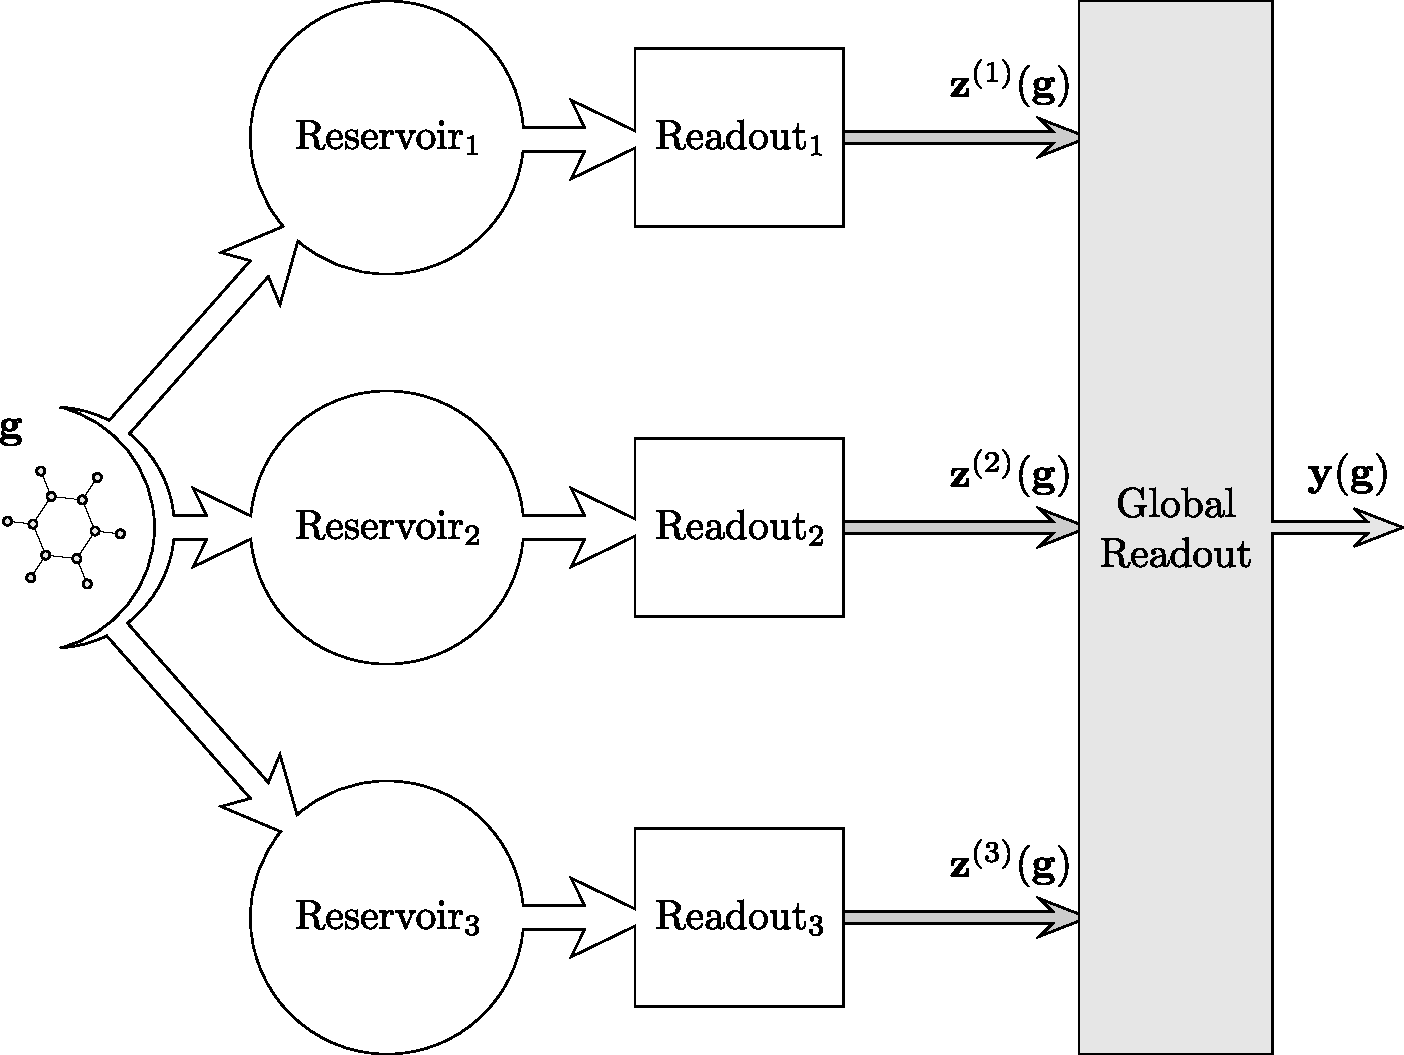
\includegraphics[width=0.8\columnwidth]{img/Modello-CF}
\medskip
\caption[GraphESN-CF.]{Modello GraphESN-CF. Topologia con tre sotto-reti.}
\label{fig:modelli:cf}
\end{figure}


\subsubsection*{GraphESN-FW}
Il modello \emph{GraphESN-FW} (i.e.\ GraphESN Forward) arricchisce il precedente attraverso una struttura più complessa. In questo caso, infatti, il readout di ogni sotto-rete riceve in input gli output-feedback provenienti dalle sotto-reti precedenti. Il risultato è una struttura in cascata in cui, in maniera simile a quanto accade per la Cascade Correlation (si veda il paragrafo~\ref{sec:intro:cnn:ccorr}), ogni sotto-rete forma un livello a sé stante dipendente dai precedenti. Poiché gli output-feedback vanno da una sotto-rete a tutte le successive, le connessioni si sviluppano ``in avanti''.

La figura~\vref{fig:modelli:fw} mostra la topologia del modello GraphESN-FW, con le connessioni in avanti.

Alcune osservazioni sono opportune riguardo alla presenza di output-feedback ed alla particolare scelta di una struttura a cascata in avanti. L'esistenza di output-feedback, infatti, determina implicitamente una relazione di dipendenza fra le varie unità computazionali (i.e.\ per poter svolgere la propria elaborazione, ogni sotto-rete necessita dell'output delle sotto-reti dalle quali riceve output-feedback). La struttura a cascata in avanti individua dunque un ordinamento parziale che mette il modello nelle condizioni di poter funzionare, determinando anche una strategia di esecuzione specifica (i.e.\ gli output vengono calcolati in sequenza, a partire dalla prima sotto-rete in poi).\\
Il fatto che gli output-feedback siano solo in avanti ha anche il vantaggio di mantenere inalterate tutte quelle sotto-reti per cui siano già state svolte delle elaborazioni, con l'effetto pratico di poter salvare i risultati ottenuti (e.g.\ l'encoding dei singoli input da parte dei reservoir) e risparmiare dunque risorse di calcolo.

\begin{figure}[p]
\centering
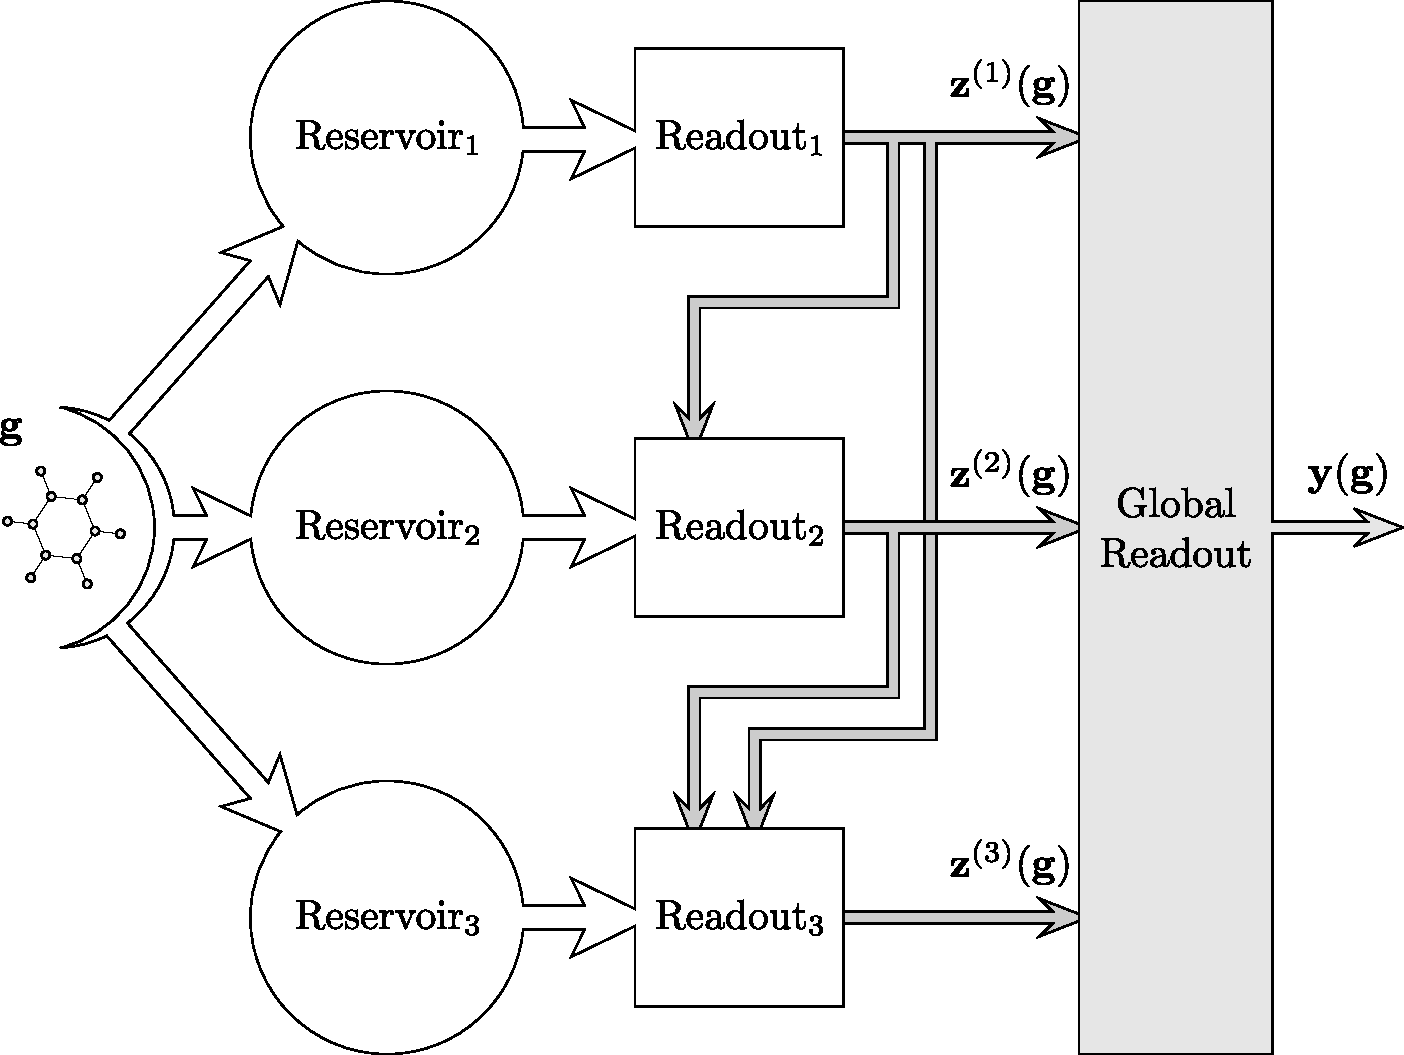
\includegraphics[width=0.8\columnwidth]{img/Modello-FW}
\medskip
\caption[GraphESN-FW.]{Modello GraphESN-FW. Topologia con tre sotto-reti.}
\label{fig:modelli:fw}
\end{figure}

\begin{figure}[p]
\centering
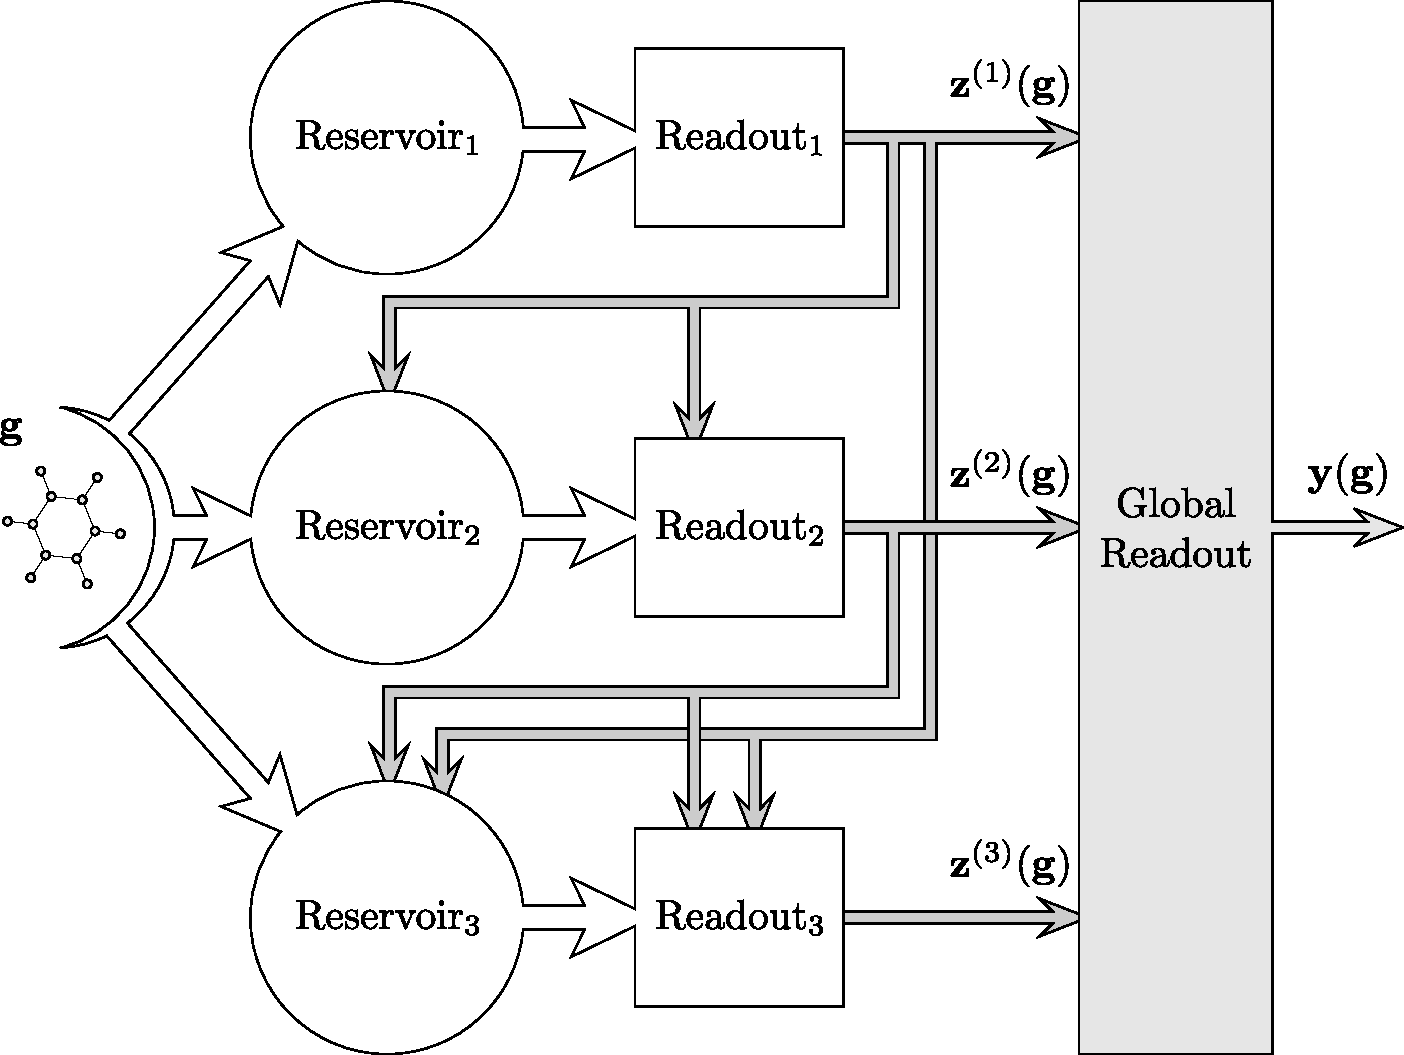
\includegraphics[width=0.8\columnwidth]{img/Modello-FOF}
\medskip
\caption[GraphESN-FOF.]{Modello GraphESN-FOF. Topologia con tre sotto-reti.}
\label{fig:modelli:fof}
\end{figure}

\subsubsection*{GraphESN-FOF}
L'ultimo modello proposto, \emph{GraphESN-FOF} (i.e.\ Graph\-ESN Forward Output-Feedback), e combina l'approccio incrementale, la struttura a cascata in avanti e l'uso degli output-feedback per spostare gli stati del reservoir come discusso nel paragrafo~\ref{sec:modelli:constr:outfeedback}. In questo caso, dunque, le connessioni in avanti sono mandate sia al readout che al reservoir di tutte le sotto-reti successive.

La struttura delle connessioni del modello GraphESN-FOF è mostrata nella figura~\ref{fig:modelli:fof}. La figura~\vref{fig:modelli:evoluzione} mostra invece i primi tre passi del processo incrementale di costruzione di una rete.


\begin{figure}[p]
\centering
\subfloat[][Struttura della rete dopo una iterazione.]
{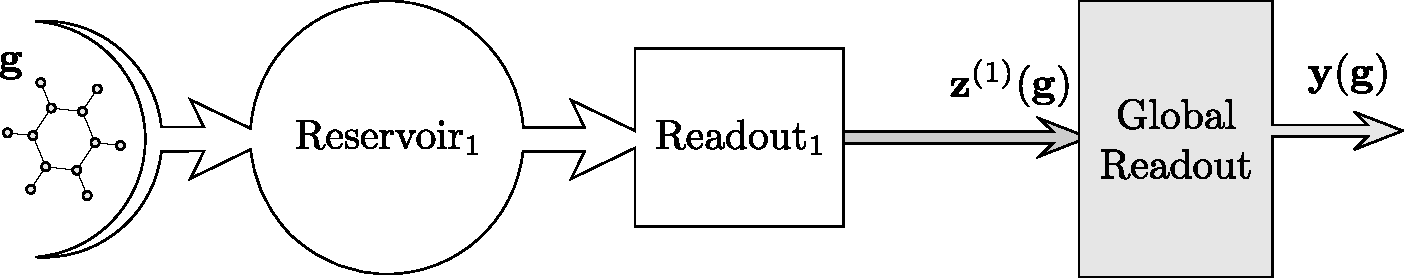
\includegraphics[width=0.75\columnwidth]{img/evoluzione1}}\\
\vspace*{0.4cm}
\subfloat[][Struttura della rete dopo due iterazioni.]
{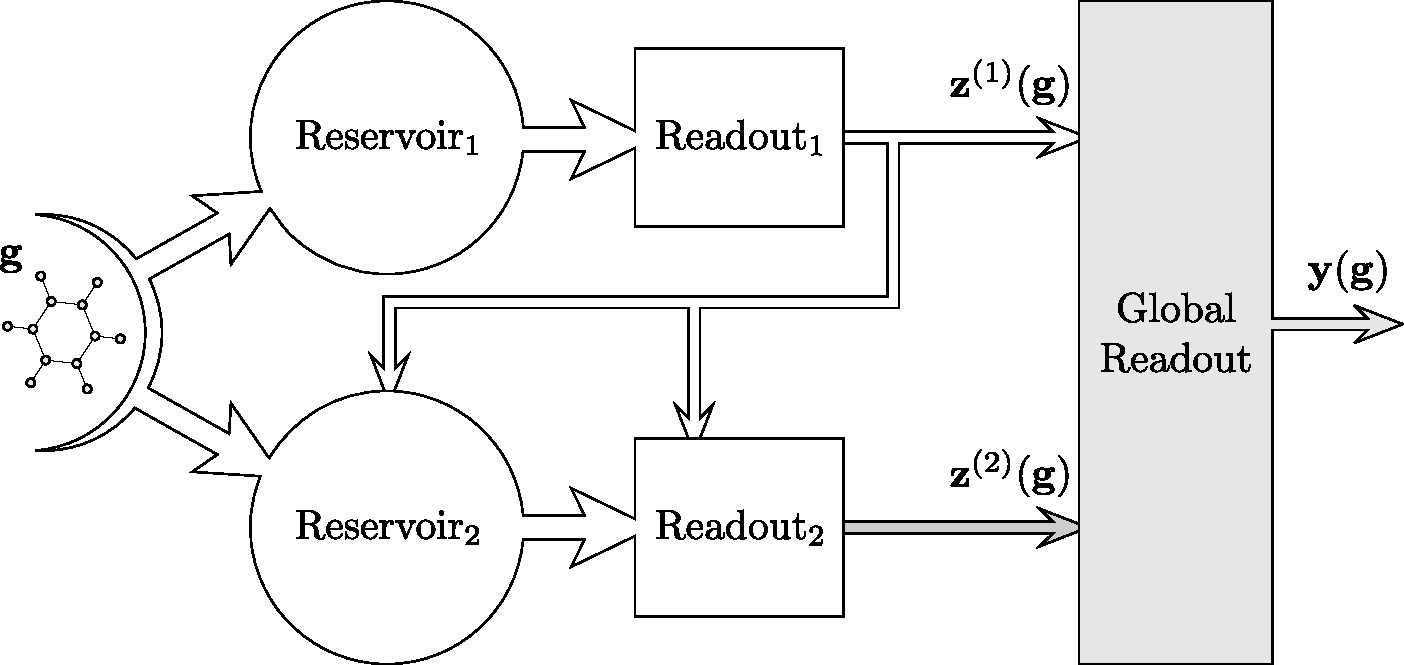
\includegraphics[width=0.75\columnwidth]{img/evoluzione2}}\\
\vspace*{0.4cm}
\subfloat[][Struttura della rete dopo tre iterazioni.]
{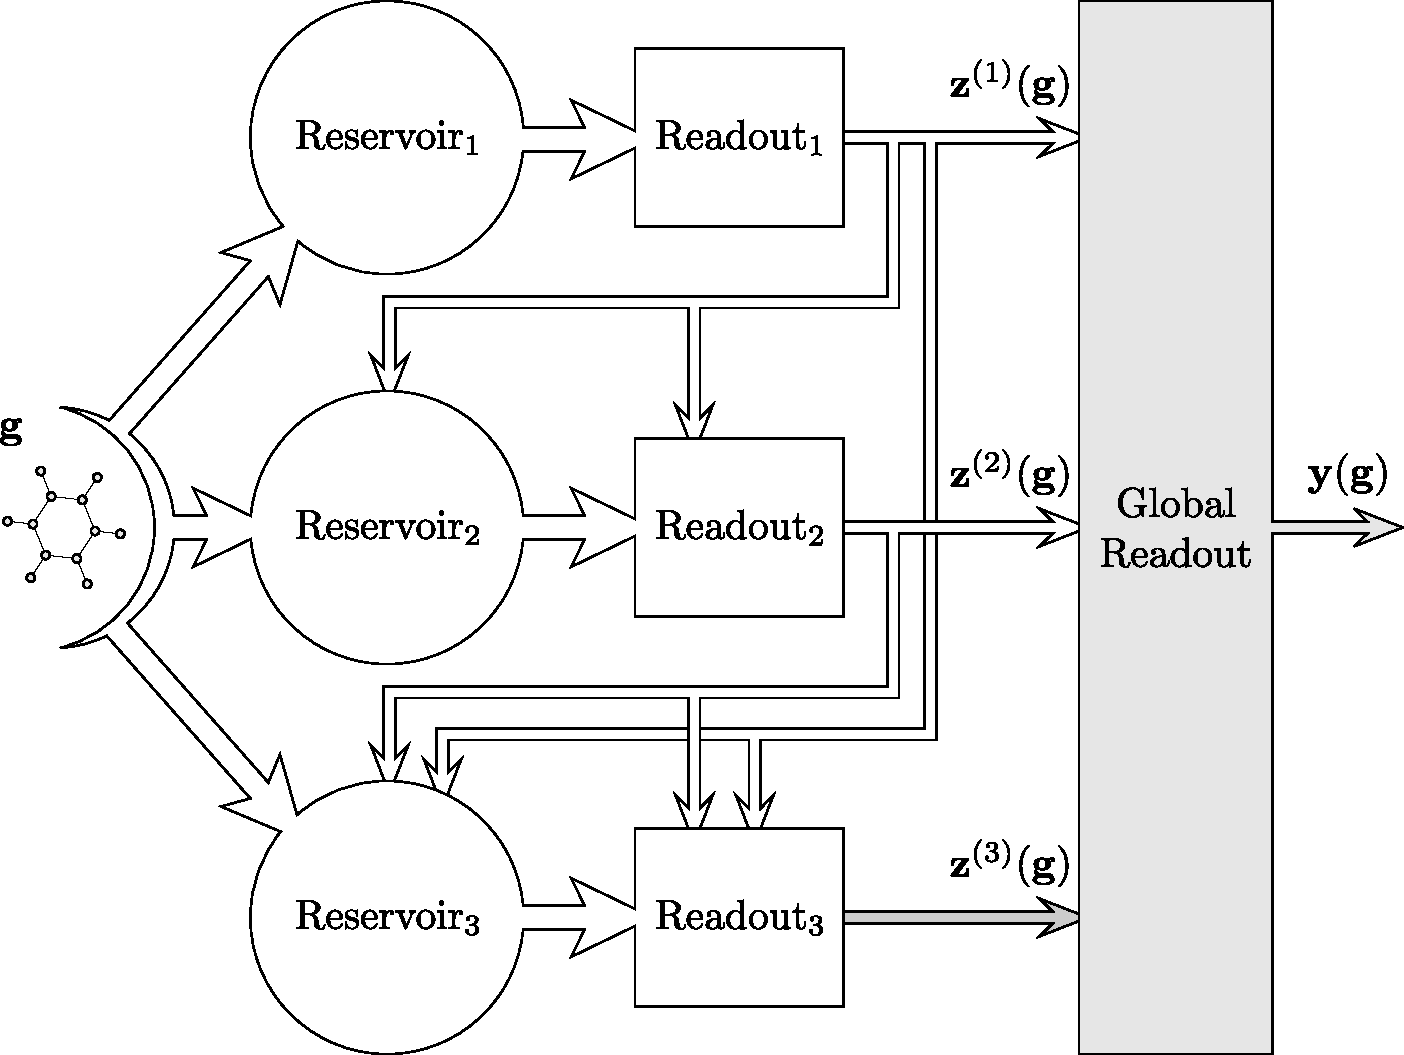
\includegraphics[width=0.75\columnwidth]{img/evoluzione3}}
\vspace*{0.4cm}
\medskip
\caption[Costruzione di una rete.]{Costruzione di una rete di tipo GraphESN-FOF. Dall'alto verso il basso, tre passi successivi di costruzione della rete. Ad ogni iterazione sono mostrate in grigio le connessioni soggette ad allenamento.}
\label{fig:modelli:evoluzione}
\end{figure}


%%%%%%%%%%%%%%%%%%%%%%%%%%%%%%%%%%
\section{Costo computazionale}\label{sec:modelli:costo}
Consideriamo una rete di tipo GraphESN-FOF formata da $\mathit{NSN}$ sotto-reti, ognuna con $N_R$ unità nel reservoir. Assumiamo inoltre, secondo un'ipotesi tutt'altro che irrealistica, che la dimensione dell'output della rete e delle sotto-reti sia trascurabile (tipicamente $N_Y = N_Z = 1$). Di seguito viene riportato il costo computazionale delle fasi principali che caratterizzano l'evoluzione della rete (si veda l'algoritmo~\vref{alg:modelli:constr}). Il dettaglio del calcolo del costo computazionale è riportato nell'appendice~\ref{app:costo}.

\subsubsection*{Encoding}
Ogni sotto-rete deve far convergere il proprio reservoir per ogni input $\graph{g} \in \mathcal{G}$ e quindi ottenere l'encoding corrispondente nello spazio delle features. Grazie alle caratteristiche dei modelli sperimentati è sufficiente che ogni sotto-rete esegua questa fase una sola volta per ogni input. 

Chiamando $\mathit{MAXV}$ il numero massimo di vertici di un grafo del dataset $\mathcal{G}$ (i.e.\ $\mathit{MAXV} = \max(\{ \abs{V(\graph{g})},\, \graph{g} \in \mathcal{G} \})$) e $\mathit{MAXIT}$ il numero massimo di iterazioni consentite per la convergenza di un singolo reservoir, il costo computazionale complessivo del processo di encoding risulta essere
\begin{equation}
	O( \mathit{NSN}\ \mathit{MAXIT}\ \mathit{MAXV}\ \abs{\mathcal{G}}\ N_R^2 )
\end{equation}
Il costo totale della codifica degli input scala quindi quadraticamente rispetto alle dimensioni del reservoir. \`E opportuno tuttavia osservare che, nel caso dei modelli proposti, la possibilità di scomporre il task in sotto-task permette l'adozione di sotto-reti di dimensioni contenute.
\\
Come nel caso delle GraphESN standard questa fase è identica sia per gli input usati nel training della rete che per il test.

Benché negli esperimenti riportati nel seguito (capitolo~\ref{ch:esperimenti}) siano stati utilizzati reservoir completamente connessi, sfruttando la presenza di sotto-reti di dimensioni contenute, il costo computazionale dell'encoding può essere ridotto assumendo una connettività sparsa nel reservoir. Nel caso in cui ogni unità del abbia al più $M$ connessioni in ingresso, il costo dell'encoding diventa
\begin{equation}
	O( \mathit{NSN}\ \mathit{MAXIT}\ \mathit{MAXV}\ \abs{\mathcal{G}}\ N_R\ M )
\end{equation}
e dipende dunque linearmente dalla dimensione dell'input e dei reservoir utilizzati.

La fase di encoding realizzata tramite i modelli proposti si caratterizza dunque, come nel caso delle GraphESN (si veda anche il paragrafo~\ref{sec:intro:struct:gesn}), per efficienza computazionale se confrontata con altri modelli per il trattamento di domini strutturati. 
Particolarmente interessante può essere in questo caso il confronto con tecniche basate su kernel: l'uso di kernel su grafi \cite{Frohlich:AssignmentKernels} comporta infatti un costo almeno quadratico rispetto al numero di vertici dell'input, e realizza un encoding non adattivo, secondo metriche prefissate. Con i modelli introdotti risulta invece possibile, ad un costo computazionale vantaggioso, realizzare la codifica dell'input tenendo conto anche dell'informazione supervisionata derivante dagli output-feedback.

I dettagli del calcolo per il costo computazionale dell'encoding sono riportati nel paragrafo~\ref{app:costo:encoding}.

\subsubsection*{Training}
Distinguiamo due distinte fasi di training, in accordo con la strategia costruttiva descritta in precedenza: il training di una singola sotto-rete e l'allenamento del readout-globale. Poiché il training riguarda in ogni caso l'adattamento dei pesi di un unico livello di connessioni, verso il readout, vari algoritmi possono essere efficacemente applicati. Nel seguito saranno considerate solo le strategie utilizzate nell'analisi sperimentale dei modelli.

Una sotto-rete può essere allenata per emulare l'errore commesso dal readout-globale. In questo caso, ricorrendo all'algoritmo di Ridge Regression (si veda il paragrafo~\ref{intro:alg}) il costo computazionale complessivo è 
\begin{multline}
	O( \mathit{NSN}^4 + N_R\ \mathit{NSN}^3 + N_R^2\ \mathit{NSN}^2 + N_R^3\ \mathit{NSN} \\ 
	+ \mathit{NSN}^3\ \abs{\mathcal{G}} + \mathit{NSN}^2\ N_R\ \abs{\mathcal{G}} + \mathit{NSN}\ N_R^2\ \abs{\mathcal{G}} )
\end{multline}
e scala dunque con il numero di sotto-reti elevato alla quarta e con il cubo della dimensione del reservoir, secondo una dipendenza critica nel determinare il vantaggio computazionale, come verrà discusso nel seguito.

Il readout-globale della rete può a sua volta essere allenato tramite Ridge Regression, con un costo complessivo
\begin{equation}
	O( \mathit{NSN}^4 + \mathit{NSN}^3 \abs{\mathcal{G}} )
\end{equation}
\`E tuttavia possibile allenare il readout-globale con Least Mean Squares (si veda il paragrafo~\ref{intro:alg}). Sia $\mathit{LMSIT}$ il numero massimo di iterazioni necessarie alla convergenza dell'algoritmo, il costo complessivo è 
\begin{equation}
	O( \mathit{LMSIT}\ \abs{\mathcal{G}}\ \mathit{NSN}^2\ )
\end{equation}
In questo caso la dipendenza è quadratica rispetto al numero complessivo di sotto-reti.

Il calcolo completo del costo computazionale dell'allenamento delle sotto-reti tramite Ridge Regression è riportato nel paragrafo~\ref{app:costo:tr_sub}, mentre i paragrafi~\ref{app:costo:tr_globale_ridge} e \ref{app:costo:tr_globale_lms} riportano il calcolo del costo per l'allenamento del readout globale tramite Ridge Regression e LMS rispettivamente.

\subsubsection*{Calcolo dell'output}
Ogni volta che una nuova sotto-rete viene allenata ed aggiunta alla rete è necessario procedere con il calcolo dell'output relativo ad ognuno dei grafi nel dataset $\mathcal{G}$. Nell'intero processo di costruzione della rete il costo del calcolo dell'output, a livello delle sotto-reti, risulta 
\begin{equation}
	O(\mathit{NSN}\ N_R\ \abs{\mathcal{G}} + \mathit{NSN}^2\ \abs{\mathcal{G}})
\end{equation}
presentando una dipendenza quadratica rispetto al numero di sotto-reti e lineare rispetto alla dimensione del dataset e del reservoir.
\`E opportuno in questo caso sottolineare come, per una generica sotto-rete, il calcolo dell'uscita dipenda dagli output-feedback delle sotto-reti precedenti, i cui valori sono precalcolati, e dal risultato della fase di encoding, anch'esso già calcolato durante la fase di allenamento.

Ad ogni incremento delle dimensioni della rete è inoltre necessario ottenere l'errore commesso dal readout-globale e quindi calcolare l'output della rete. Poiché il readout-globale prende in input unicamente gli output delle singole sotto-reti il costo complessivo è
\begin{equation}
	O(\mathit{NSN}^2\ \abs{\mathcal{G}})
\end{equation}
e scala linearmente con la dimensione del dataset e quadraticamente rispetto al numero di sotto-reti.

Il dettaglio del calcolo del costo computazionale per ottenere l'output delle sotto-reti e del readout globale è riportato nei paragrafi~\ref{app:costo:out_sub} e \ref{app:costo:out_globale} rispettivamente.

\subsubsection*{Costo complessivo}
In riferimento ad una GraphESN-FOF, con reservoir completamente connesso, che usi l'algoritmo Ridge Regression per l'apprendimento, è  possibile riassumere il costo computazionale delle singole fasi come indicato nella tabella~\ref{tab:modelli:costo}.

\begin{table}[htbp]
\small
\centering
\caption{Costo computazionale di GraphESN-FOF}
\label{tab:modelli:costo}
\begin{tabular}{>{\scshape }p{.3\textwidth} >{$\displaystyle}p{.6\textwidth}<{$}}
\toprule
Encoding & O( \mathit{NSN}\ \mathit{MAXIT}\ \mathit{MAXV}\ \abs{\mathcal{G}}\ N_R^2 ) \\[0.1cm]
Learning (SubNets) & \hspace*{-0.18cm}
\begin{array}{l}
O(\mathit{NSN}^4 + N_R\ \mathit{NSN}^3 + N_R^2\ \mathit{NSN}^2 + N_R^3\ \mathit{NSN}  \\
	\quad + \mathit{NSN}^3\ \abs{\mathcal{G}} + \mathit{NSN}^2\ N_R\ \abs{\mathcal{G}} + \mathit{NSN}\ N_R^2\ \abs{\mathcal{G}}) \\
\end{array}\\ [0.2cm]
Learning (Global) & O(\mathit{NSN}^4 + \mathit{NSN}^3 \abs{\mathcal{G}}) \\ [0.1cm]
Output (SubNets) & O(\mathit{NSN}\ N_R\ \abs{\mathcal{G}} + \mathit{NSN}^2\ \abs{\mathcal{G}}) \\ [0.1cm]
Output (Global) & O(\mathit{NSN}^2\ \abs{\mathcal{G}}) \\ [0.1cm]
\bottomrule
\end{tabular}
\end{table}




%%%%%%%%%%%%%%%%%%%%%%%%%%%%%%
\subsection{Considerazioni}
I modelli di Reservoir Computing sono caratterizzati, in generale, per l'efficienza computazionale. La possibilità di limitare l'allenamento alle sole unità del readout, facendo affidamento sulle caratteristiche strutturali del reservoir per realizzare l'encoding, permette infatti l'impiego di algoritmi di apprendimento semplici e computazionalmente poco onerosi. Per poter efficacemente riflettere sul costo computazionale dei modelli proposti è dunque opportuno guardare a questo ambito, prendendo come riferimento il confronto con la GraphESN standard (si veda il paragrafo~\ref{sec:intro:struct:gesn}), che i modelli estendono.

Per le varie fasi di utilizzo di una GraphESN, assumendo anche in questo caso l'adozione di reservoir completamente connessi e formati da un numero totale di unità pari a quelle di tutte le sotto-reti di una GraphESN-FOF (i.e.\ $N_R' = N_R\, \mathit{NSN}$), possiamo considerare il costo computazionale riportato nella tabella~\ref{tab:modelli:costo_gesn}. 

\begin{table}[htbp]
\small
\centering
\caption{Costo computazionale di una GraphESN con $N_R' = N_R\, \mathit{NSN}$.}
\label{tab:modelli:costo_gesn}
\begin{tabular}{>{\scshape }p{.15\textwidth} >{$\displaystyle}p{.45\textwidth}<{$}}
\toprule
Encoding & O((N_R\, \mathit{NSN})^2\ \mathit{MAXIT}\ \mathit{MAXV}\ \abs{\mathcal{G}}) \\[0.1cm]
Learning & O((N_R\, \mathit{NSN})^3 + (N_R\, \mathit{NSN})^2 \ \abs{\mathcal{G}}) \\ [0.1cm]
Output   & O(\abs{\mathcal{G}}\ N_R\ \mathit{NSN}) \\ [0.1cm]
\bottomrule
\end{tabular}
\end{table}

Le differenze principali emergono, confrontando il costo delle GraphESN con quello dei modelli costruttivi, osservando la dipendenza del costo computazionale rispetto alle dimensioni del reservoir. 
La dipendenza quadratica del processo di encoding delle GraphESN rispetto a $\mathit{NSN}$ diventa infatti lineare con l'adozione della strategia costruttiva. Il costo dell'apprendimento, che nelle GraphESN dipende dal cubo del prodotto di $\mathit{NSN}$ ed $N_R$, è a sua volta ridotto di due ordini di grandezza rispetto a $\mathit{NSN}$.
Di contro, sia per l'apprendimento che per il calcolo dell'output, le reti costruttive presentano un costo fortemente dipendente dal numero di sotto-reti, che determina uno svantaggio nel caso in cui il valore di $\mathit{NSN}$ domini sugli altri.

%Nel caso costruttivo, il processo di encoding scala con il quadrato di $N_R$ mentre per le GraphESN 
%L'impiego della strategia costruttiva permette infatti di ridurre l'impatto di $N_R$ di un ordine di grandezza sia nella fase di encoding che in quella di apprendimento. Di contro, in entrambi i casi il costo computazionale risulta legato al numero di sotto-reti secondo una relazione che cresce con la quarta potenza, determinando uno svantaggio nel caso in cui il valore di $\mathit{NSN}$ domini sugli altri.

\begin{figure}[tb]
\centering
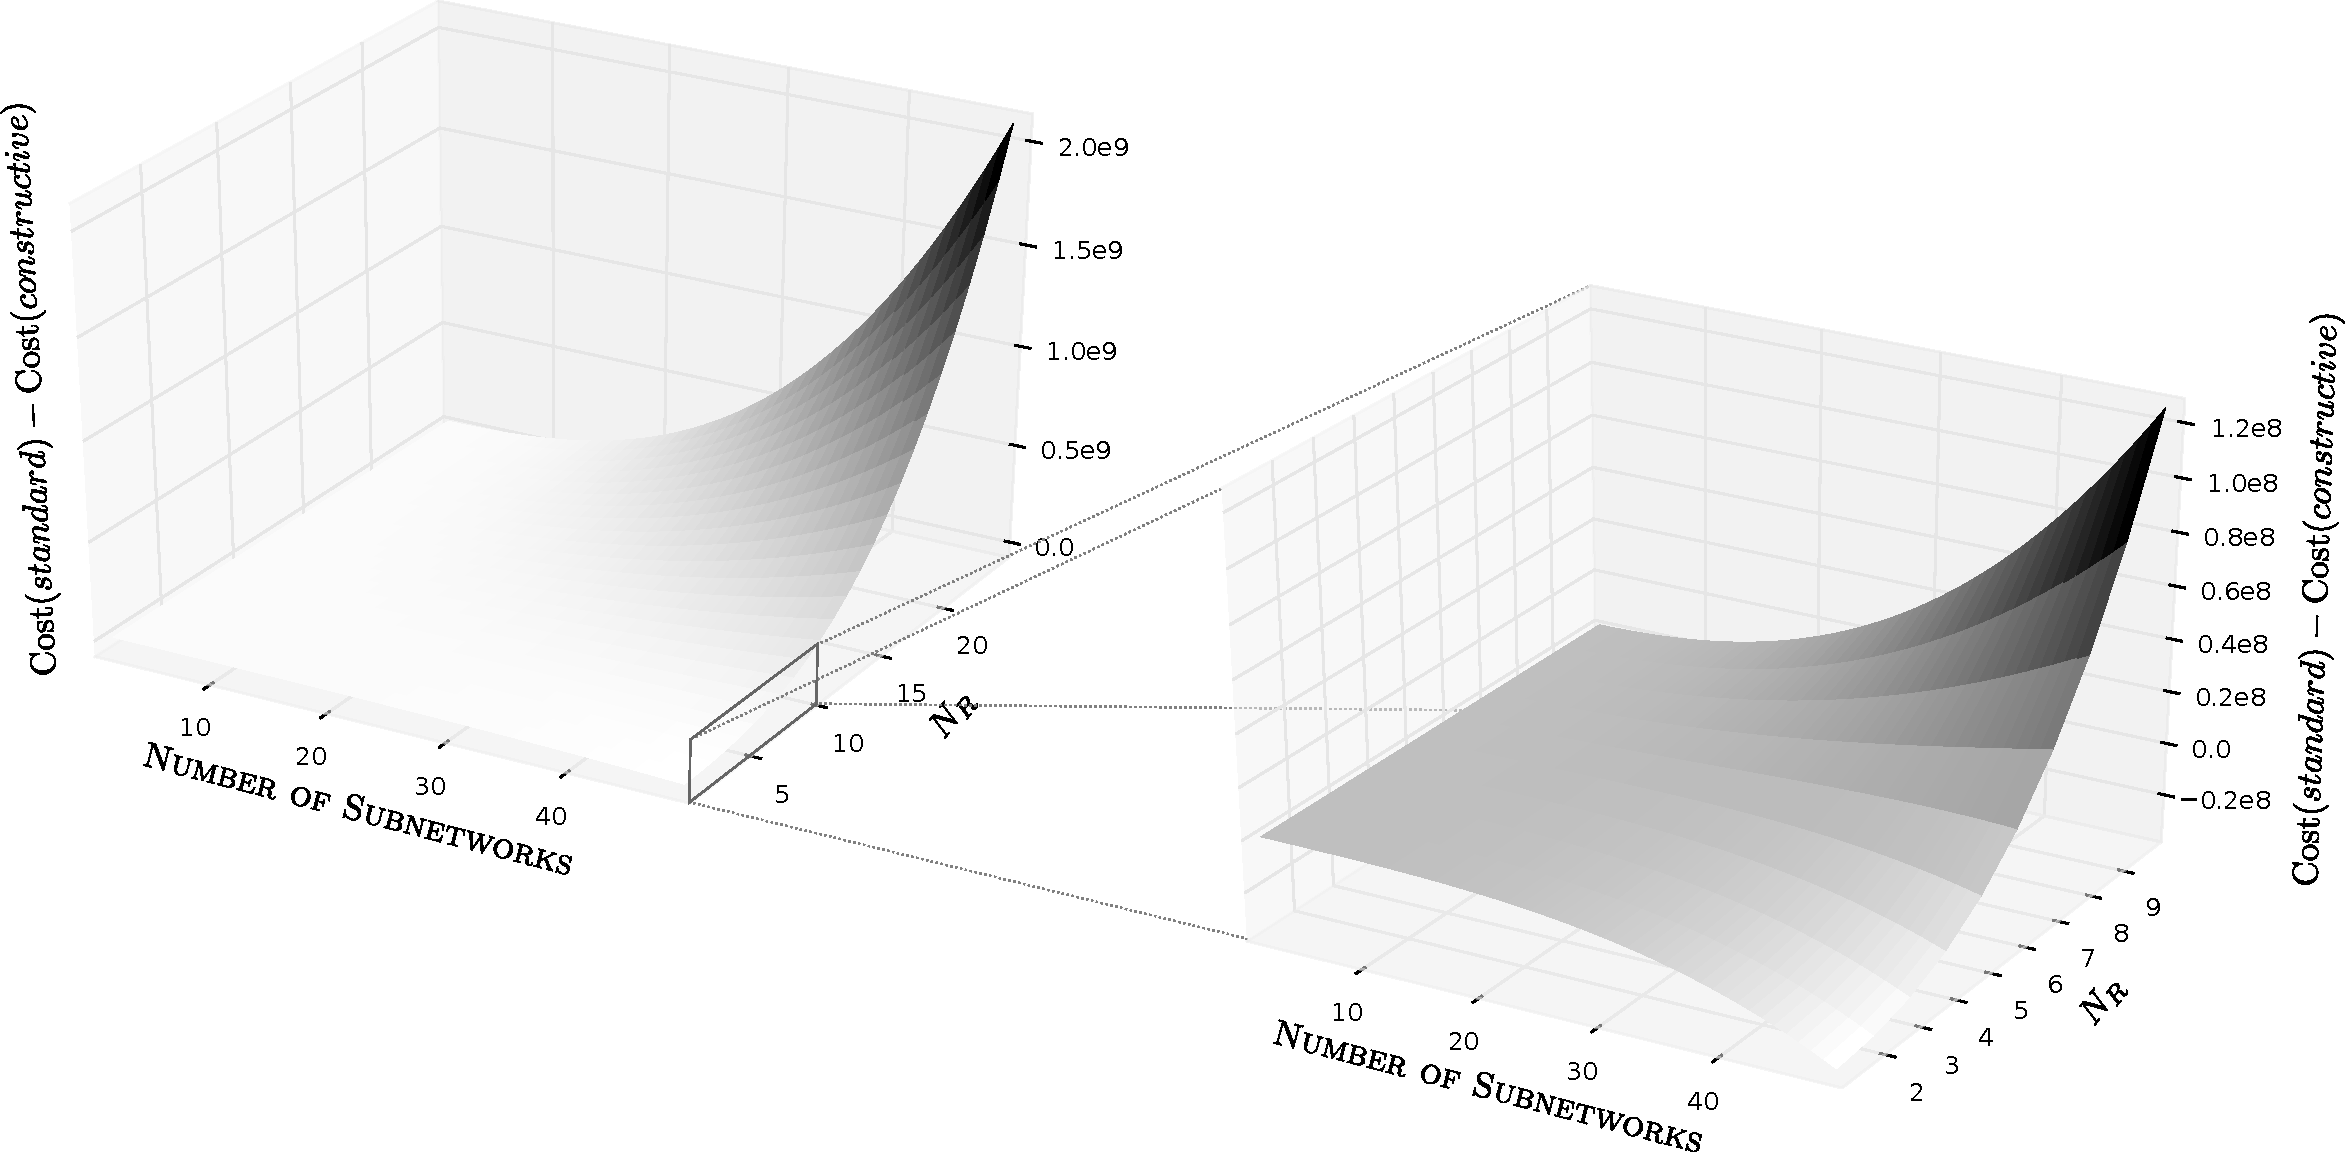
\includegraphics[width=1.0\columnwidth]{img/costo-v2}
\medskip
\caption[Approccio costruttivo: vantaggio computazionale]{Vantaggio computazionale nell'uso dell'approccio costruttivo. Assi orizzontali: numero di sotto-reti e dimensioni del reservoir ($N_R$). Asse verticale: differenza fra costo del modello standard e costo del modello costruttivo.\\
(\emph{sx}) $N_R \in [1,25]$. (\emph{dx}) Dettaglio della regione con minore vantaggio computazionale: $N_R \in [1,10]$.}
\label{fig:modelli:costo}
\end{figure}

La figura~\vref{fig:modelli:costo} dà un'intuizione di quale sia il vantaggio dal punto di vista computazionale derivato dall'adozione dell'approccio costruttivo. A parità di dimensioni del dataset (i.e.\ $\abs{\mathcal{G}} = 100$ ) ed al variare delle dimensioni dei reservoir e del numero delle sotto-reti, la figura mostra come varia la differenza fra il costo di una GraphESN standard equivalente (i.e.\ con reservoir di dimensione $N_R' = N_R\, \mathit{NSN}$) e di una GraphESN-FOF. I valori positivi corrispondono dunque ai casi in cui l'approccio costruttivo risulta più efficiente.\\
La figura evidenzia come con il crescere delle dimensioni dei reservoir ed all'aumentare del numero di sotto-reti, l'approccio costruttivo risulti in un vantaggio computazionale notevole. 
La possibilità di scomporre un problema in sotto-problemi si rispecchia infatti nella struttura complessiva della rete, che impiega, rispetto al caso delle GraphESN, più reservoir di dimensioni ridotte, il cui allenamento richiede un impiego minore di risorse di calcolo.
A destra nella figura è evidenziata tuttavia l'esistenza di particolari condizioni per le quali l'impiego di una strategia costruttiva risulta essere sconveniente. Tale situazione si verifica in particolare nel caso in cui si usino molte sotto-reti di dimensioni estremamente ridotte. La motivazione risiede nel fatto che, in un simile scenario, il costo computazionale complessivo risulta dominato dal processo iterativo di costruzione della rete piuttosto che dalla dimensione dei reservoir trattati. 
In merito a quanto detto è tuttavia opportuno osservare che, per la natura stessa del Reservoir Computing, l'impiego di reservoir con un numero davvero esiguo di unità è da considerarsi poco realistico.

Un'ulteriore osservazione risulta particolarmente importante per valutare i modelli proposti dal punto di vista computazionale. Benché il confronto con una singola GraphESN lasci emergere i vantaggi dei modelli proposti, è infatti opportuno sottolineare come la strategia costruttiva comporti particolari benefici anche in termini di selezione del modello. Per determinare la corretta dimensione della rete, infatti, i modelli non costruttivi si affidano ad un approccio \emph{trial and error} in cui ogni possibile variazione nella dimensione del reservoir viene allenata e valutata in maniera indipendente. Al contrario, l'approccio costruttivo permette di determinare la dimensione della rete in maniera automatica ed offre quindi l'opportunità di ridurre di molto il numero di esperimenti necessari a determinare quali siano gli iperparametri più adatti per la risoluzione di un task. \\
Intuitivamente possiamo dunque dire che il costo speso per la costruzione incrementale di una singola rete costruttiva, corrisponda all'allenamento ed il test di svariate reti diverse nel caso delle GraphESN. Per fare un esempio possiamo pensare che l'allenamento di una GraphESN-FOF, formata da $\mathit{NSN}$ sotto-reti di dimensione $N_R$, corrisponda, in termini computazionali, all'allenamento di $\mathit{NSN}$ diverse GraphESN, con reservoir di dimensioni crescenti: $N_R' \in \lbrace N_R, 2 N_R, \dots, \mathit{NSN}\, N_R \rbrace$.
Questo porta ad avere un costo complessivo per la selezione di una GraphESN pari a (si veda il paragrafo~\ref{app:costo:modelselection})
\begin{multline}
O(\mathit{NSN}^4\ N_R^3 + \mathit{NSN}^3\ N_R^2\ \mathit{MAXIT}\ \mathit{MAXV}\ \abs{\mathcal{G}} \\
+ \mathit{NSN}^3\ N_R^2\ \abs{\mathcal{G}} + \mathit{NSN}^2\ N_R\ \abs{\mathcal{G}}) 
\end{multline}
che scala con il prodotto fra $N_R^3$ e $\mathit{NSN}^4$ determinando una dipendenza estremamente svantaggiosa rispetto al caso dell'allenamento di una singola GraphESN-FOF, in cui i due fattori compaiono congiunti in una dipendenza al più quadratica.

Quanto detto evidenzia dunque come i modelli proposti si caratterizzino per efficienza dal punto di vista computazionale. La strategia costruttiva introdotta permette infatti di ridurre gli oneri del processo di apprendimento rispetto alle GraphESN, già di per sé contraddistinte dall'efficienza computazionale, rispondendo ad un'esigenza molto rilevante nell'ambito del trattamento dei domini strutturati. 
\`E infine opportuno sottolineare come l'utilizzo di uno schema di output-feedback permetta, nei modelli proposti, di influenzare il processo di encoding in maniera supervisionata senza che questo comporti la perdita, in termini computazionali, dei vantaggi derivati dall'uso di un reservoir non adattivo.



%%%%%%%%%%%%%%%%%%%%%%%%%%%%%%
\section{Software}\label{ch:modelli:software}
Un'implementazione software dei modelli descritti nel corso del capitolo è stata realizzata utilizzando il linguaggio \texttt{Python}\footnote{\url{http://python.org/}} (versione 2.6). 

Essendo un linguaggio dinamico, dalla sintassi semplice e fornito di un'ampia libreria standard, \texttt{Python} risulta particolarmente efficace per la prototipazione rapida. Questa caratteristica è stata considerata particolarmente desiderabile ai fini della realizzazione del lavoro svolto. Lo sviluppo dei modelli, così come quello del software, è infatti stato portato avanti in maniera incrementale, secondo un percorso guidato anche dall'esito di prove empiriche e sperimentali.

La scelta del linguaggio è risultata inoltre soddisfacente in termini di performance, nonostante il fatto che \texttt{Python} sia un linguaggio interpretato. L'utilizzo della libreria \texttt{scipy}\footnote{\url{http://www.scipy.org/}} per l'algebra lineare ha infatti permesso di raggiungere prestazioni comparabili con quelle ottenibili realizzando gli stessi modelli in \texttt{MATLAB}\footnote{\url{http://www.mathworks.com/products/matlab/}}, il cui utilizzo è ampiamente diffuso nell'ambito della realizzazione di modelli neurali.

Il software sviluppato sarà rilasciato con licenza open source.


%%%%%%%%%%%%%%%%%%%%%%%%%%%%%%%%%%%%%%%%%%%%%%%%%%%%%%%%%%%%%%%%%%%%%%%%%%%%%%%%
%%%%%%%%%%%%%%%%%%%%%%%%%%%%%%%%%%%%%%%%%%%%%%%%%%%%%%%%%%%%%%%%%%%%%%%%%%%%%%%%


\begin{comment}
Consideriamo una rete (FOF) formata da 'd' sotto-reti. Tutti i reservoir hanno
dimensione Nr, sia le sotto-reti che il readout-globale hanno output Ny, che
però è trascurabile.

--------------------------------------------------------------------------------

*** Convergenza del reservoir ***

La rete i-esima

    x_t(v) = f(Win u(v) + \sum_{w} W x_{t-1}(w) + Wfof z(g))

con:
    Win     :   (Nr, Nu)
    W       :   (Nr, Nr)
    Wfof    :   (Nr, Ny * (i-1))

Per un grafo g:
    Win u(v)                :   O(Nr Nu |V(g)|) - calcolato una sola volta
    Wfof z(g)               :   O(Nr Ny (i+1))  - calcolato una volta sola
    \sum_{w} W x_{t-1}(w)   :   O(Nr^2 |V(g)|)  - ad ogni iterazione

Chiamiamo 'j' il numero massimo di iterazioni e 'v' il numero massimo di 
vertici.
Il calcolo viene ripetuto per ogni grafo, quindi |G| volte.
La convergenza del reservoir i-esimo sull'intero grafo quindi costa:

    O(|G| (Nr Nu v + Nr Ny (i-1) + Nr^2 v j))
    ~ O(|G| Nr^2 v j)

gli output-feedback risultano trascurabili: quello che pesa è il processo 
iterativo del reservoir.
Il costo della convergenza di *tutte* le sotto-reti è dunque 'd' volte quello
di una singola sotto-rete:

    O(d |G| Nr^2 v j)


--------------------------------------------------------------------------------

*** Training (sotto-rete) ***

** Con Max-S
Per ogni iterazione (rete i-esima):
    Calcolo dell'output                         :   O(|G| (Nr + Ny (i-1)) Ny)
    Calcolo correlazione                        :   O(|G| Ny)
    Calcolo \sigma_o (E_po - \bar{E}_o) f'_p    :   O(|G| Ny)
    Calcolo gradiente                           :   O(|G| (Nr + Ny (i-1)) Ny) 

Mettendo tutto insieme, un'iterazione costa:

    O(|G| Ny (2 + (Nr + Ny (i-1))))
    ~ O(|G| Ny Nr + |G| i Ny^2)

Chiamiamo 'q' il numero massimo di iterazioni necessarie alla convergenza.
Il costo complessivo per l'applicazione dell'algoritmo a *tutte* le sotto-reti è

    O(q d |G| Ny Nr + q |G| Ny^2 d^2)
    ~ O(q d |G| Nr + q |G| d^2)         [Ny trascurabile]


** Con Ridge-Regression

    W.T = (A.T A + \lambda I)^-1 A.T B

con 

    A   :   (|G|, Nr + Ny (i-1)) = (|G|, Nf) 
    B   :   (|G|, Ny)

ho chiamato Nf = Nr + Ny (i-1) il numero di features in input al readout. E'
solo per comodità (n.b. Nf varia a sotto-rete a sotto-rete).

Costo:
    A.T A                           :   O(Nf^2 |G|)     [prodotto]
    (A.T A + \lambda I)^-1          :   O(Nf^3)         [inversione]
    A.T B                           :   O(Nf |G| Ny)    [prodotto]
    (A.T A + \lambda I)^-1 A.T B    :   O(Nf^2 Ny)      [prodotto]

Mettendo tutto insieme:

    O(Nf^3 + Nf^2 |G| + Nf^2 Ny + Nf |G| Ny)
    ~ O(Nf^3 + Nf^2 |G| + Nf^2 + Nf |G|)        [Ny trascurabile]
    ~ O(Nf^3 + Nf^2 |G|)

Cechiamo di calcolare il costo per tutta la rete, ovvero per 'd' sotto-reti.
Quanto vale Nf? Per l'unità i-esima: Nf = Nr + Ny (i-1)
Quindi:

Nf_1 = Nr
Nf_2 = Nr + Ny
Nf_3 = Nr + 2 Ny
Nf_4 = Nr + 3 Ny
...
Nf_d = Nr + (d-1) Ny

Quindi:

(Nf_1)^2 = Nr^2
(Nf_2)^2 = Nr^2 + Ny^2 + 2 Nr Ny
(Nf_3)^2 = Nr^2 + 4 Ny^2 + 4 Nr Ny
(Nf_3)^2 = Nr^2 + 9 Ny^2 + 6 Nr Ny
...
(Nf_d)^2 = Nr^2 + (d-1)^2 Ny^2 + 2 (d-1) Nr Ny

sommando: O(d Nr^2 + Ny^2 d^3  + Nr Ny d^2) 
            ~ O(d^3 + d^2 Nr + d Nr^2)      [Ny trascurabile]

Passiamo al cubo:

(Nf_1)^3 = Nr^3
(Nf_2)^3 = Nr^3 + Ny^3 + 3 Nr^2 Ny + 3 Nr Ny^2
(Nf_3)^3 = Nr^3 + 8 Ny^3 + 6 Nr^2 Ny + 12 Nr Ny^2
(Nf_3)^3 = Nr^3 + 27 Ny^3 + 9 Nr^2 Ny + 27 Nr Ny^2
...
(Nf_d)^3 = Nr^3 + (d-1)^3 Ny^3 + 3 (d-1) Nr^2 Ny + 3 (d-1)^2 Nr Ny^2

sommando: O(d Nr^3 + Ny^3 d^4 + Nr^2 Ny d^2 + Nr Ny^2 d^3)
            ~ O(d^4 + Nr d^3 + Nr^2 d^2 + Nr^3 d)       [Ny trascurabile]

Mettendo tutto insieme, il costo del training di tutte le sotto-reti tramite
ridge-regression è

    O(d^4 + Nr d^3 + Nr^2 d^2 + Nr^3 d + d^3 |G| + d^2 Nr |G| + d Nr^2 |G|)



--------------------------------------------------------------------------------

*** Training (readout-globale) ***

** Con Ridge-Regression

Come il caso precedente, ma senza alcun reservoir (i.e.\ solo gli output-feedback
in input)

    O(Nf^3 + Nf^2 |G|) con Nf = Ny (i-1) per la sotto-rete i-esima

Quindi:

    O(Ny^3 d^4 + Ny^2 d^3 |G|)
    ~ O(d^4 + d^3 |G|)          [Ny trascurabile]


** Con LMS

Per un singolo allenamento, dopo aver aggiunto la sotto-rete i-esima:

    O(|G| Nf Ny) = O(r |G| (i-1) Ny^2)

con 'r' numero massimo di iterazioni per la convergenza.

Complessivamente il costo è:

    O(r |G| d^2 Ny^2)
    ~ O(r |G| d^2)    [Ny trascurabile]


--------------------------------------------------------------------------------

*** Calcolo dell'output (sotto-rete) ***

Tutti i valori in input sono precalcolati (reservoir + output-feedback).
Il costo è quello della moltiplicazione:

    Wout [X(x(g)), z_1(g), ... , z_{i-1}(g)] = Wout in

con:
    Wout    :   (Ny, Nr + Ny (i-1))
    in      :   Nr + Ny (i-1)

Quindi per una rete ed un input:

    O(Ny (Nr + Ny (i-1)))
    = O(Ny Nr + Ny^2 (i-1))

Il costo del calcolo dell'output di *tutte* le 'd' sotto-reti è dunque:

    O(|G| ((Ny Nr) + (Ny Nr + Ny^2) + (Ny Nr + 2 Ny^2) + ... + (Ny Nr + (d-1) Ny^2))))
    = O(|G| (d Ny Nr + Ny^2 d^2))
    ~ O(d Nr |G| + d^2 |G|)         [Ny trascurabile]


--------------------------------------------------------------------------------

*** Calcolo dell'output (readout globale) ***

Differisce dal caso precedente solo perché ha in input unicamente gli 
output-feedback, quindi nessun reservoir.

    O(Ny^2 d^2 |G|)
    ~ O(d^2 |G|)


********************************************************************************
********************************************************************************

*** Confronto: Costruttivo VS Standard ***

** GraphESN Costruttiva

reservoir:          O(d |G| Nr^2 v j)
sub learning:       O(d^4 + Nr d^3 + Nr^2 d^2 + Nr^3 d + d^3 |G| + d^2 Nr |G| + d Nr^2 |G|) 
gloabl learning:    O(d^4 + d^3 |G|) 
sub output:         O(d Nr |G| + d^2 |G|) 
global output:      O(d^2 |G|) 

** GraphESN Stadard

reservoir:          O(d |G| Nr^2 v j) (???) O(|G| (d Nr)^2 )
learning:           O(Nr^3 + Nr^2 |G|)
output:             O(|G| Nr)

\end{comment}


